\documentclass[a4paper,12pt]{report}

\usepackage[utf8]{inputenc}
\usepackage[T1]{fontenc}
\usepackage{array}
\usepackage{amsmath}
\usepackage[english]{babel}
\usepackage{graphicx}
\usepackage[a4paper]{geometry}
\usepackage[colorlinks=true,urlcolor=blue,linkcolor=blue]{hyperref}
\usepackage{url}
\usepackage[nottoc,numbib]{tocbibind}
\usepackage{color}
\usepackage{epstopdf}
\usepackage{xcolor}
\usepackage[backend=biber,style=phys]{biblatex}

\addbibresource{../Bibliography.bib}

\makeatletter
	\renewcommand{\thechapter}{\Roman{chapter}}
\makeatother

\begin{document}

\chapter{Dynamics of a single Cr spin in a ZnTe quantum dot}

%	\section{Experiment configuration}
	\section{Experimental setup}	
	
%		\subsection{Experimental setup}
		
	\begin{figure}[h!]
	\begin{center}
		\includegraphics[width=10cm]{../FillingPicture.png}
	\end{center}
	\caption{Complete experimental setup with three lasers, accousto-modulator, finishing either on the monochromator or the diodes.}
	\label{ExpSetup}
	\end{figure}
	
	Lorem ipsum dolor sit amet, consectetur adipiscing elit. Curabitur tortor quam, imperdiet quis facilisis sed, fringilla a quam. Cras ante odio, hendrerit ac ante nec, cursus imperdiet urna. Mauris convallis ultricies purus, nec condimentum erat bibendum vel. Aliquam erat volutpat. Pellentesque condimentum, eros a consequat accumsan, turpis sem euismod nisi, sed fringilla quam turpis sit amet erat. Mauris dictum odio sed nisi dapibus, et molestie mauris rutrum. Praesent convallis dolor in nibh blandit bibendum. Quisque sit amet arcu consectetur lorem luctus venenatis nec quis dui. Aliquam erat volutpat. Aenean auctor elit nec tristique dignissim. Nulla massa mi, efficitur semper ex id, pretium eleifend massa. Vivamus sit amet orci scelerisque, gravida est ut, vulputate odio.
		
%		\subsection{Studied dot}
		
%	\begin{figure}[h!]
%	\begin{center}
%		\includegraphics[width=10cm]{../FillingPicture.png}
%	\end{center}
%	\caption{Studied dot spectra and linear polarization}
%	\label{DotSpectra}
%	\end{figure}
%	
%	Lorem ipsum dolor sit amet, consectetur adipiscing elit. Curabitur tortor quam, imperdiet quis facilisis sed, fringilla a quam. Cras ante odio, hendrerit ac ante nec, cursus imperdiet urna. Mauris convallis ultricies purus, nec condimentum erat bibendum vel. Aliquam erat volutpat. Pellentesque condimentum, eros a consequat accumsan, turpis sem euismod nisi, sed fringilla quam turpis sit amet erat. Mauris dictum odio sed nisi dapibus, et molestie mauris rutrum. Praesent convallis dolor in nibh blandit bibendum. Quisque sit amet arcu consectetur lorem luctus venenatis nec quis dui. Aliquam erat volutpat. Aenean auctor elit nec tristique dignissim. Nulla massa mi, efficitur semper ex id, pretium eleifend massa. Vivamus sit amet orci scelerisque, gravida est ut, vulputate odio.
%	
%	\begin{figure}[h!]
%	\begin{center}
%		\includegraphics[width=10cm]{../FillingPicture.png}
%	\end{center}
%	\caption{Spectra with different excitation and detection configurations}
%	\label{ExpConfig}
%	\end{figure}
%	
%	Lorem ipsum dolor sit amet, consectetur adipiscing elit. Curabitur tortor quam, imperdiet quis facilisis sed, fringilla a quam. Cras ante odio, hendrerit ac ante nec, cursus imperdiet urna. Mauris convallis ultricies purus, nec condimentum erat bibendum vel. Aliquam erat volutpat. Pellentesque condimentum, eros a consequat accumsan, turpis sem euismod nisi, sed fringilla quam turpis sit amet erat. Mauris dictum odio sed nisi dapibus, et molestie mauris rutrum. Praesent convallis dolor in nibh blandit bibendum. Quisque sit amet arcu consectetur lorem luctus venenatis nec quis dui. Aliquam erat volutpat. Aenean auctor elit nec tristique dignissim. Nulla massa mi, efficitur semper ex id, pretium eleifend massa. Vivamus sit amet orci scelerisque, gravida est ut, vulputate odio.
	
	\section{Cr spin time fluctuations}
	
		\subsection{Autocorrelation: conservation of the Cr spin}
		
	\begin{figure}[h!]
	\begin{center}
		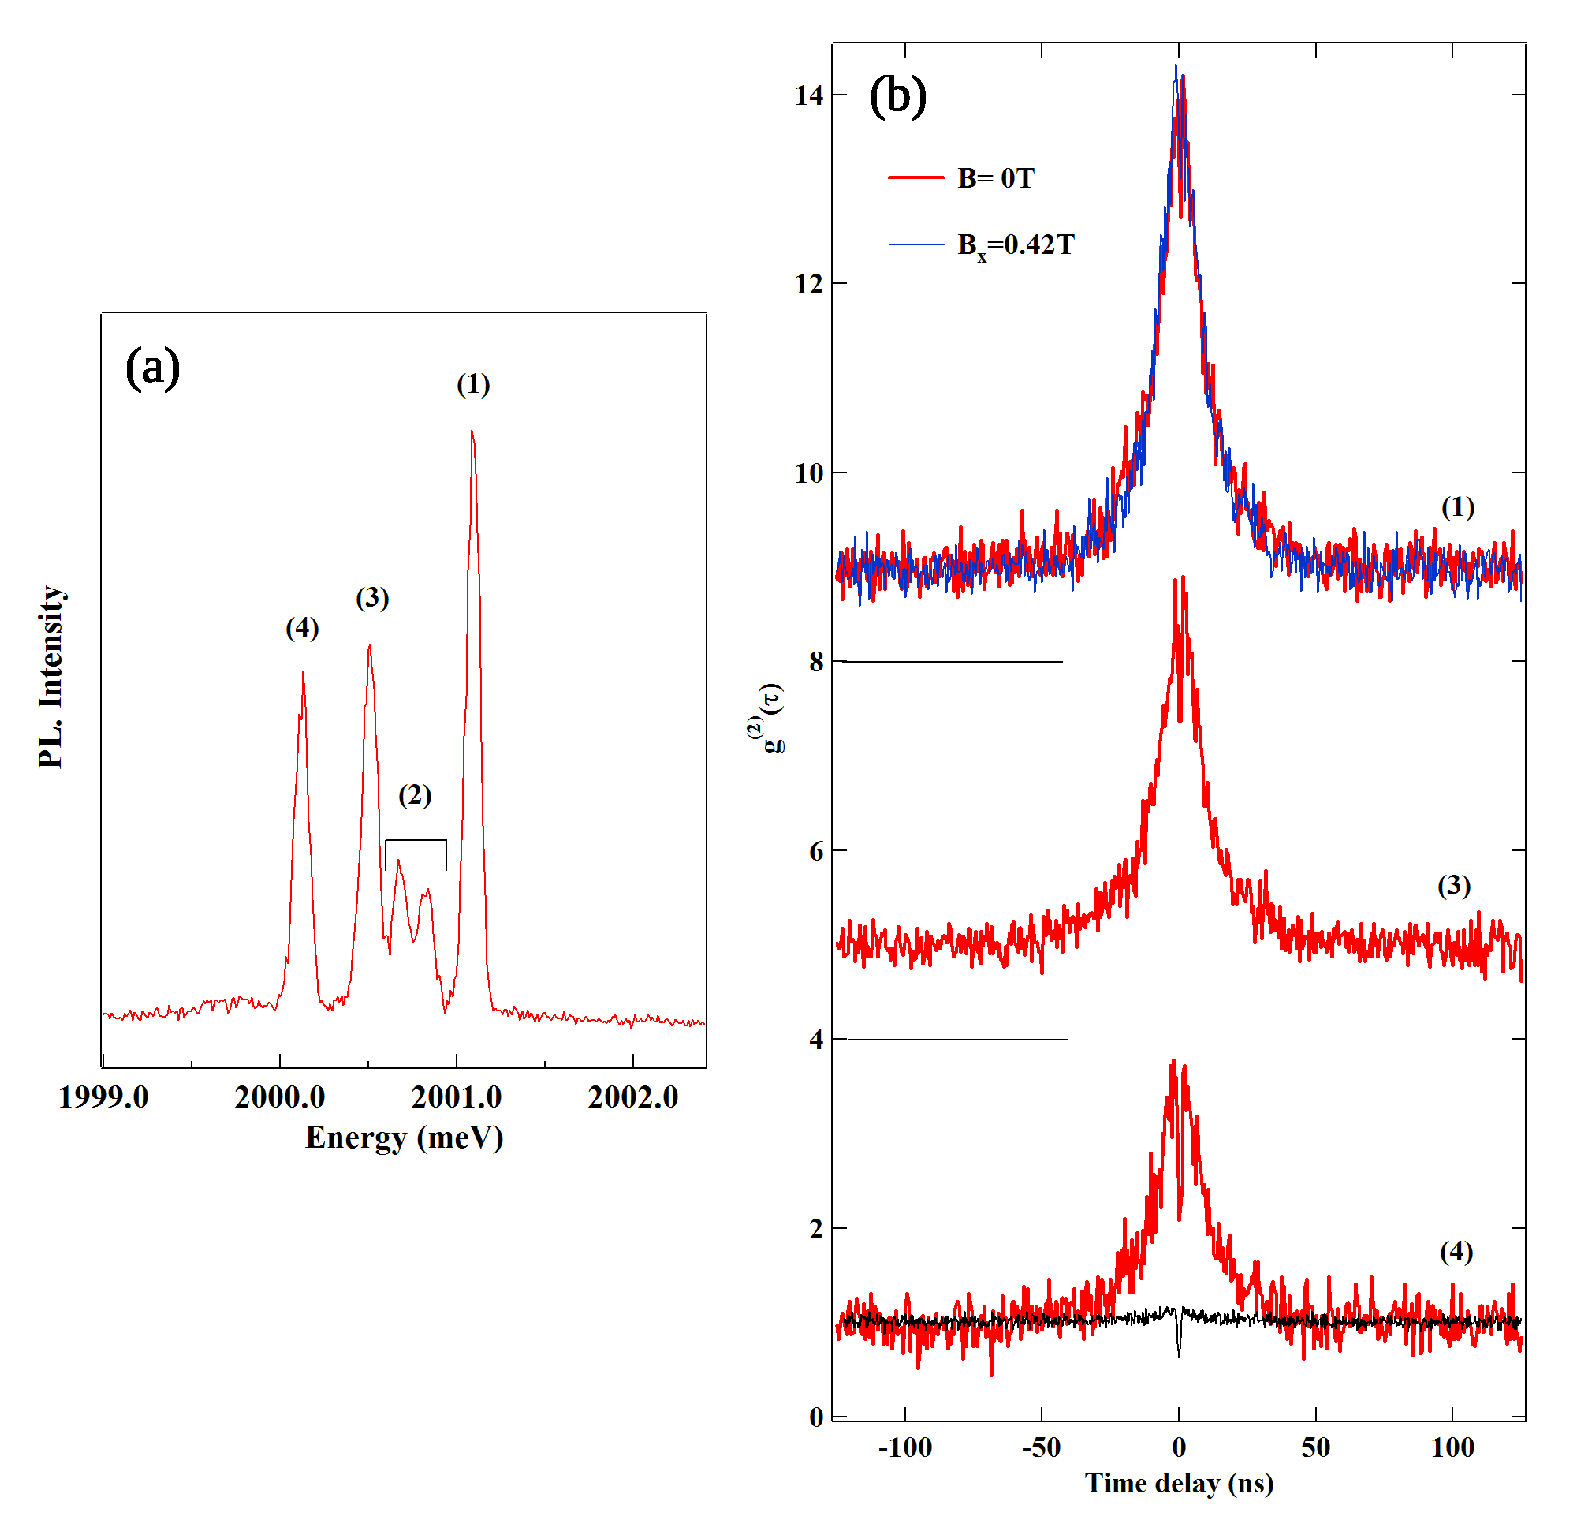
\includegraphics[width=10cm]{Pictures/AutocorPeaks.eps}
	\end{center}
	\caption{Autocor of X alone in comparison of X-Cr, and autocor of 3 peaks with comparison with and without B field}
	\label{AutocorExpCr}
	\end{figure}		
		
		To observe the time fluctuations of the Cr spin under CW optical excitation, we used the statistics of time arrivals of the photons emitted by a Cr-doped QD given by the second order correlation function g$^{(2)}(\tau)$ of the PL intensity. Fig.~\ref{AutocorExpCr} shows g$^{(2)}(\tau)$ for the lines (1), (3) and (4) recorded in circular polarization. These signals are compared with the auto-correlation obtained for the PL of a non-magnetic QD which is characteristic of a single-photon emitter with a dip (anti-bunching) at short delays. The width of the anti-bunching is given by the lifetime of the emitter and the generation rate of excitons and its depth is limited by the time resolution of the HBT setup. As illustrated in Fig.~\ref{AutocorExpCr}, typical non-magnetic CdTe/ZnTe QDs do not present any significant bunching induced by charge fluctuations \cite{QDAutocor,IndistPhoton}. A similar auto-correlation on a X-Cr PL line still presents a reduced coincidence rate near zero delay, but it is mainly characterized by a large photon bunching with a full width at half maximum (FWHM) in the 20 ns range. This large bunching reflects an intermittency in the emission of a given line of the QD coming from fluctuations of the Cr spin in a 10 ns timescale as it will be confirmed by cross-correlation measurements.

The amplitude of the bunching reaches 5 for line (1) and is slightly weaker for the lower energy lines. In a simple picture of blinking where the selected QD line can be either in a state ON or OFF, the amplitude of the bunching is given by $\Gamma_{OFF}/\Gamma_{ON}$, ratio of the transition rates from OFF to ON, $\Gamma_{ON}$, and from ON to OFF, $\Gamma_{OFF}$ \cite{SubnanoSpectDiff}. An amplitude of bunching larger than 1 is then expected in a multilevel spin system where, after a spin relaxation, multiple spin-flips are usually required to come back to the initial state ($\Gamma_{ON}<\Gamma_{OFF}$). Let us finally note that the bunching signal is not affected by a weak transverse magnetic field ($B_x=0.42$T in Fig.~\ref{AutocorExpCr}). This confirms the presence of a large strain induced magnetic anisotropy $D_0$ which splits the Cr and X-Cr states and blocks their precession in a magnetic field.

	\begin{figure}[h!]
	\begin{center}
		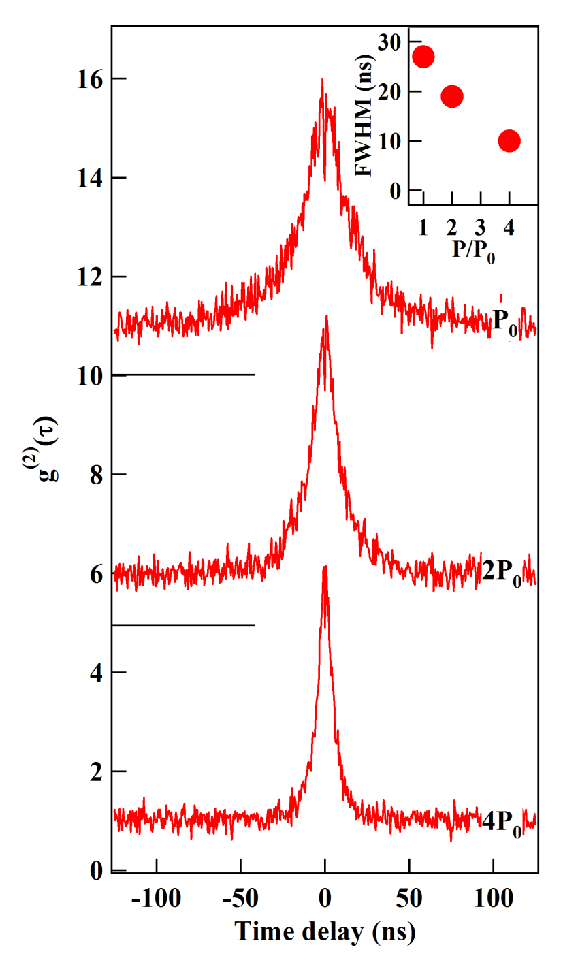
\includegraphics[width=6cm]{Pictures/AutocorPw.eps}
	\end{center}
	\caption{Autocor power variation effect}
	\label{AutocorPwCr}
	\end{figure}	

	Curabitur eget ipsum egestas dui viverra suscipit. Cras aliquet lacus vitae erat finibus semper. Nulla pharetra eget urna vitae sodales. Nunc faucibus velit lacus, nec ornare eros aliquet quis. Donec a orci nec sem pulvinar ultricies sit amet ut arcu. Nullam id vehicula enim, at tincidunt velit. Duis vestibulum lorem a molestie fringilla. Nullam tincidunt semper placerat. Donec nibh sem, ornare eget cursus ac, luctus sit amet eros. Phasellus eget interdum nisi. Donec mollis risus id lectus fringilla, et commodo risus iaculis. Donec at lacus sed nibh posuere posuere sit amet eget sapien. In dignissim, enim sit amet convallis fermentum, lacus nulla gravida tortor, non facilisis ex nisl sit amet augue. Maecenas eu enim condimentum, consectetur ligula vel, tincidunt nisl. Nam laoreet dictum volutpat. Donec at erat venenatis, ultrices lorem ac, vestibulum neque.
	
		
		\subsection{Cross-correlation: flipping of the Cr spin}
		
		Lorem ipsum dolor sit amet, consectetur adipiscing elit. Curabitur tortor quam, imperdiet quis facilisis sed, fringilla a quam. Cras ante odio, hendrerit ac ante nec, cursus imperdiet urna. Mauris convallis ultricies purus, nec condimentum erat bibendum vel. Aliquam erat volutpat. Pellentesque condimentum, eros a consequat accumsan, turpis sem euismod nisi, sed fringilla quam turpis sit amet erat. Mauris dictum odio sed nisi dapibus, et molestie mauris rutrum. Praesent convallis dolor in nibh blandit bibendum. Quisque sit amet arcu consectetur lorem luctus venenatis nec quis dui. Aliquam erat volutpat. Aenean auctor elit nec tristique dignissim. Nulla massa mi, efficitur semper ex id, pretium eleifend massa. Vivamus sit amet orci scelerisque, gravida est ut, vulputate odio.
		
	\begin{figure}[h!]
	\begin{center}
		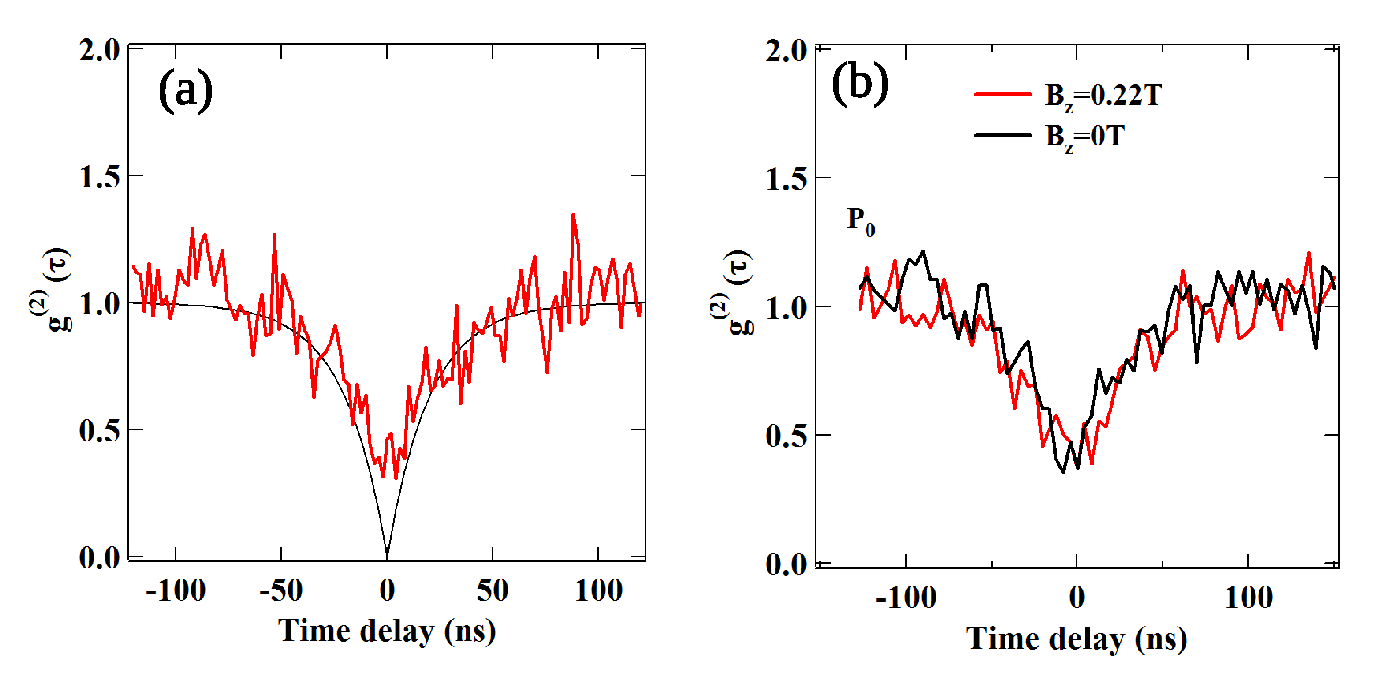
\includegraphics[width=15cm]{Pictures/CrosscorFit+B.eps}
	\end{center}
	\caption{Cross-correlation fitted with exponential, and cross correlation under magnetic field.}
	\label{CrosscorExpCr}
	\end{figure}	
		
	Curabitur eget ipsum egestas dui viverra suscipit. Cras aliquet lacus vitae erat finibus semper. Nulla pharetra eget urna vitae sodales. Nunc faucibus velit lacus, nec ornare eros aliquet quis. Donec a orci nec sem pulvinar ultricies sit amet ut arcu. Nullam id vehicula enim, at tincidunt velit. Duis vestibulum lorem a molestie fringilla. Nullam tincidunt semper placerat. Donec nibh sem, ornare eget cursus ac, luctus sit amet eros. Phasellus eget interdum nisi. Donec mollis risus id lectus fringilla, et commodo risus iaculis. Donec at lacus sed nibh posuere posuere sit amet eget sapien. In dignissim, enim sit amet convallis fermentum, lacus nulla gravida tortor, non facilisis ex nisl sit amet augue. Maecenas eu enim condimentum, consectetur ligula vel, tincidunt nisl. Nam laoreet dictum volutpat. Donec at erat venenatis, ultrices lorem ac, vestibulum neque.
	
	\begin{figure}[h!]
	\begin{center}
		\includegraphics[width=10cm]{Pictures/FillingPicture.png}
	\end{center}
	\caption{Cross-correlation under power variation}
	\label{CrosscorPwCr}
	\end{figure}	
	
	Curabitur eget ipsum egestas dui viverra suscipit. Cras aliquet lacus vitae erat finibus semper. Nulla pharetra eget urna vitae sodales. Nunc faucibus velit lacus, nec ornare eros aliquet quis. Donec a orci nec sem pulvinar ultricies sit amet ut arcu. Nullam id vehicula enim, at tincidunt velit. Duis vestibulum lorem a molestie fringilla. Nullam tincidunt semper placerat. Donec nibh sem, ornare eget cursus ac, luctus sit amet eros. Phasellus eget interdum nisi. Donec mollis risus id lectus fringilla, et commodo risus iaculis. Donec at lacus sed nibh posuere posuere sit amet eget sapien. In dignissim, enim sit amet convallis fermentum, lacus nulla gravida tortor, non facilisis ex nisl sit amet augue. Maecenas eu enim condimentum, consectetur ligula vel, tincidunt nisl. Nam laoreet dictum volutpat. Donec at erat venenatis, ultrices lorem ac, vestibulum neque.
	
		\subsection{Power dependency: relaxation paths}
		
	\begin{figure}[h!]
	\begin{center}
		\includegraphics[width=10cm]{Pictures/PwVar.eps}
	\end{center}
	\caption{Excitation power variations on dot334 QD3 and plot of the intensity of each peak}
	\label{CrSpectraPwExp}
	\end{figure}
	
	In order to study the different relaxation path of the system, probing of the emission evolution under excitation power was realized, reported on Fig.~\ref{CrSpectraPwExp}. As expected, the PL is becoming more intense with the augmentation of the excitation laser, since more exciton are produced and thus injected in the quantum dot. However, this power augmentation response is not the same for each of the peaks. The two central peaks, associated with the $|0\rangle$ states, start at about twice the intensity of the $|\pm1\rangle$ peaks for the most intense one, seemingly never reaching their maximum under our power range. However, when lowering the excitation power, they diminish quickly, and even seems to disappear at low energy, when exterior peaks still show luminescence. Plotting this evolution shows that the two central peaks exhibit a super-linear evolution. On the other side, the exterior peaks begin by rising in intensity before diminishing in a sub-linear fashion. This is coherent with the usual picture, where high power populating preferentially X$^2$-Cr states, while low power populates preferentially X-Cr states~\cite{??}. Finally, one can notice that the dark exciton exhibit the same behaviour, but the maximum emission intensity is at slightly lower power than the $|\pm1\rangle$.

	\begin{figure}[h!]
	\begin{center}
		\includegraphics[width=10cm]{Pictures/FillingPicture.png}
	\end{center}
	\caption{Power variation simulation}
	\label{CrSpectraPwMod}
	\end{figure}
	
	The results of this evolution are well reproduced by our spin effective Hamiltonian, using the parameters found for the dot from the magneto-optics and the linear polarization fitting. The model results are presented in Fig.~\ref{CrSpectraPwMod}. [NOT SURE, TO BE REDISCUSSED]The super-linear behaviour of the central peaks can be explained by the proximity of dark exciton states. High power excitation can unlock radiative recombination path to states remaining nonradiative at low excitation power~\cite{PwSuperLinInc}. Such states linked to the $|0\rangle$ state make the emission on its peaks present a super-linear behaviour when excited at high power. 		
		
		\subsection{Model of the spin dynamics}	

	\begin{figure}[h!]
	\begin{center}
		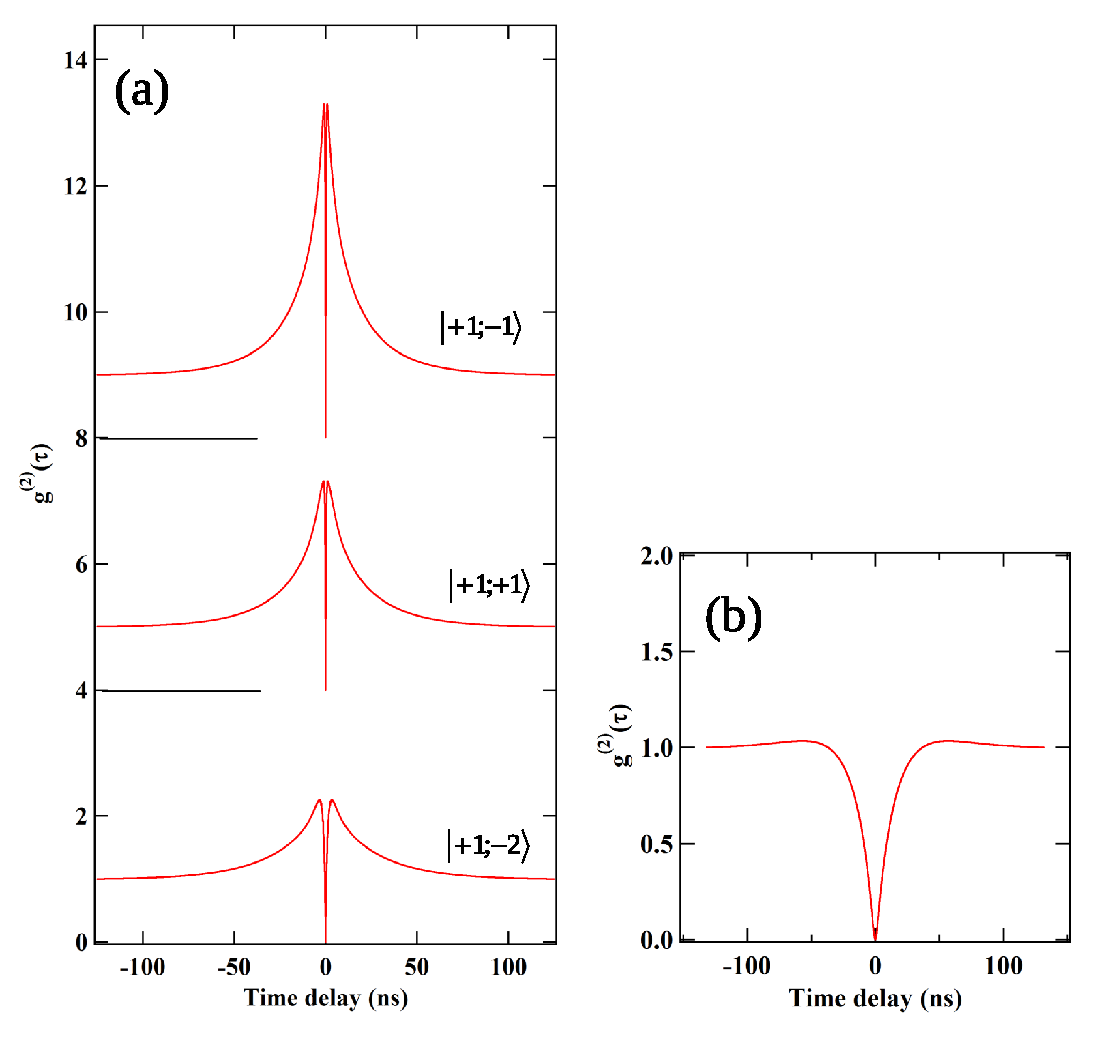
\includegraphics[width=10cm]{Pictures/SimulAutoCross.eps}
	\end{center}
	\caption{Simulation of autocorrelation on each peak and cross-correlation $|+1\rangle$ to $|+1\rangle$}
	\label{SimulCRossAuto}
	\end{figure}			
		
	To identify the main contribution to the observed spin fluctuations, we modelled the auto-correlation of the PL of X-Cr using the full spin level structure of a Cr-doped QD. We calculated the time evolution of the population of the twenty X-Cr states in the excited state of the QD and five Cr states in the ground state by solving numerically the master equation for the corresponding 25 x 25 density matrix $\rho$. The time evolution of the density matrix including relaxation and dephasing processes in the Lindblad form is given by $\partial \rho/\partial t=-i/\hbar[{\cal H},\rho]+L\rho$ where ${\cal H}$ is the Hamiltonian of the complete system ($X$-Cr and Cr) and $L\rho$ describes the coupling or decay channels resulting from an interaction with the environment \cite{SpinQJumps,ephBroad}. The energy levels of the Cr are controlled by the magnetic anisotropy $D_0S_z^2$. The X-Cr Hamiltonian, presented in Ref.\cite{LafuenteCrQD}, contains the energy of the Cr spin states, the carriers-Cr exchange interactions, the electron-hole exchange interaction in a confining potential of low symmetry and the structure of the valence band including heavy-hole/light-hole mixing. $D_0$ in the Cr Hamiltonian and the parameters in the X-Cr Hamiltonian cannot be precisely extracted from the zero magnetic field PL (Fig.~\ref{DotSpectra}(a)). For a qualitative description of the observed spin dynamics, we use in the model typical Cr-doped QD parameters extracted from magneto-optics measurements presented in Ref. \cite{LafuenteCrQD}. These parameters give a X-Cr splitting and a dark/bright excitons mixing similar to the one observed in the QD discussed in this article.
	
	\begin{figure}[h!]
	\begin{center}
		\includegraphics[width=10cm]{Pictures/FillingPicture.png}
	\end{center}
	\caption{Autocorrelation simulation with $\tau_{Cr}$ variations}
	\label{AutocorTauVar}
	\end{figure}	

	Curabitur eget ipsum egestas dui viverra suscipit. Cras aliquet lacus vitae erat finibus semper. Nulla pharetra eget urna vitae sodales. Nunc faucibus velit lacus, nec ornare eros aliquet quis. Donec a orci nec sem pulvinar ultricies sit amet ut arcu. Nullam id vehicula enim, at tincidunt velit. Duis vestibulum lorem a molestie fringilla. Nullam tincidunt semper placerat. Donec nibh sem, ornare eget cursus ac, luctus sit amet eros. Phasellus eget interdum nisi. Donec mollis risus id lectus fringilla, et commodo risus iaculis. Donec at lacus sed nibh posuere posuere sit amet eget sapien. In dignissim, enim sit amet convallis fermentum, lacus nulla gravida tortor, non facilisis ex nisl sit amet augue. Maecenas eu enim condimentum, consectetur ligula vel, tincidunt nisl. Nam laoreet dictum volutpat. Donec at erat venenatis, ultrices lorem ac, vestibulum neque.
	
	\begin{figure}[h!]
	\begin{center}
		\includegraphics[width=10cm]{Pictures/FillingPicture.png}
	\end{center}
	\caption{Simulation of autocorrelation and cross-correlation under magnetic field}
	\label{AutoCrosModMagField}
	\end{figure}	
	
	Curabitur eget ipsum egestas dui viverra suscipit. Cras aliquet lacus vitae erat finibus semper. Nulla pharetra eget urna vitae sodales. Nunc faucibus velit lacus, nec ornare eros aliquet quis. Donec a orci nec sem pulvinar ultricies sit amet ut arcu. Nullam id vehicula enim, at tincidunt velit. Duis vestibulum lorem a molestie fringilla. Nullam tincidunt semper placerat. Donec nibh sem, ornare eget cursus ac, luctus sit amet eros. Phasellus eget interdum nisi. Donec mollis risus id lectus fringilla, et commodo risus iaculis. Donec at lacus sed nibh posuere posuere sit amet eget sapien. In dignissim, enim sit amet convallis fermentum, lacus nulla gravida tortor, non facilisis ex nisl sit amet augue. Maecenas eu enim condimentum, consectetur ligula vel, tincidunt nisl. Nam laoreet dictum volutpat. Donec at erat venenatis, ultrices lorem ac, vestibulum neque.
	
	\begin{figure}[h!]
	\begin{center}
		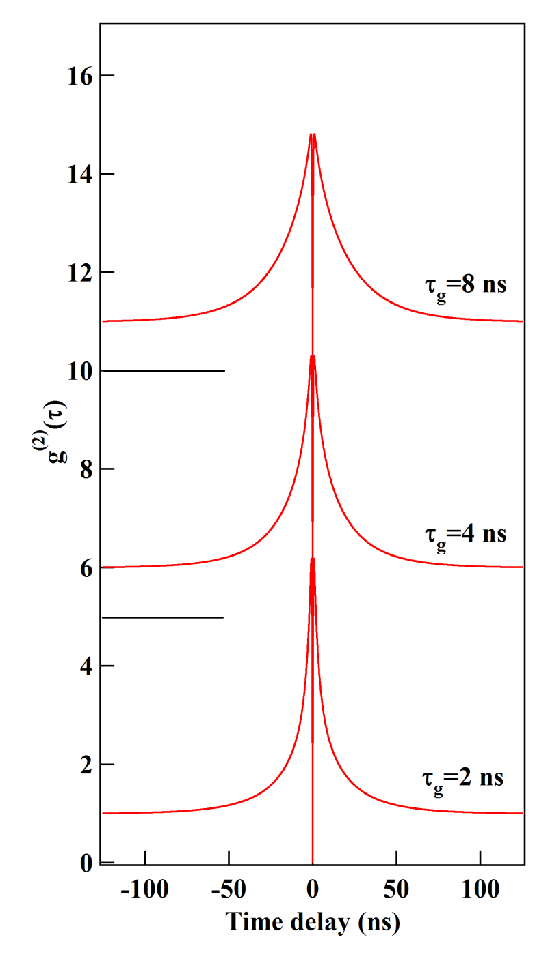
\includegraphics[width=6cm]{Pictures/SimulAutocorPw.eps}
	\end{center}
	\caption{Simulation of autocorrelation under power variation}
	\label{AutocorPwMod}
	\end{figure}			
	
	\section{Preparation the spin of a Cr atom in a quantum dot}
	
		\subsection{Resonant optical pumping of a spin level}
		
	\begin{figure}[h!]
	\begin{center}
		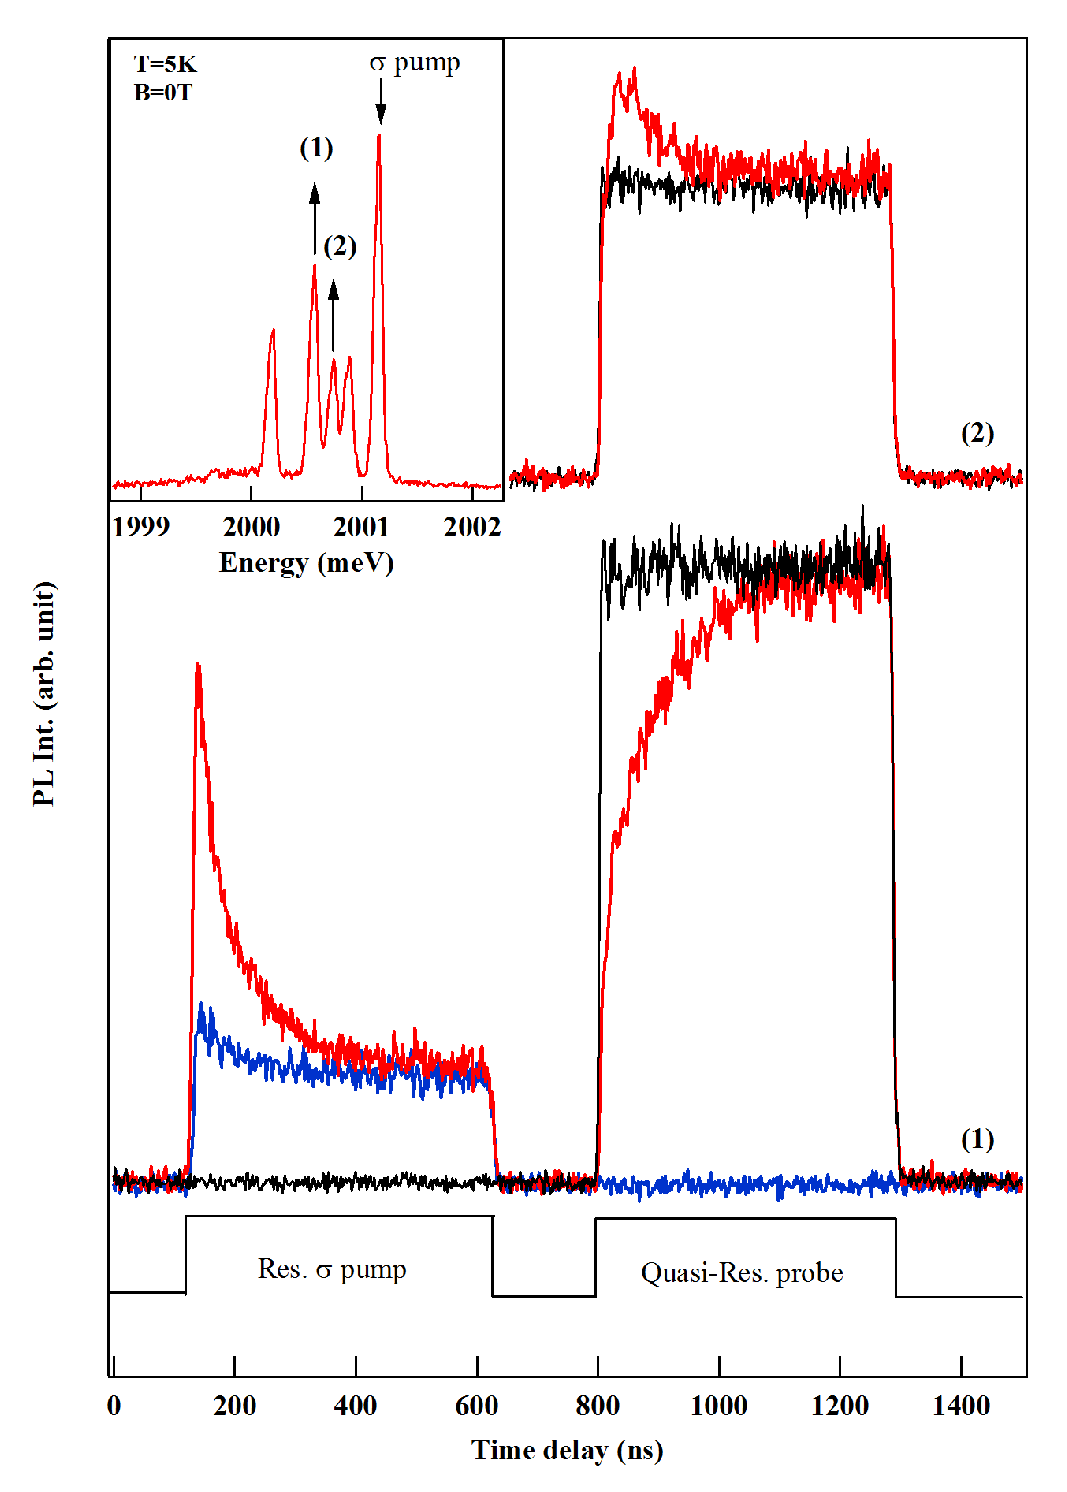
\includegraphics[width=10cm]{Pictures/Pump0+1.eps}
	\end{center}
	\caption{Pumping on peak 2 and 3}
	\label{PumpCrExp}
	\end{figure}	
	
		Lorem ipsum dolor sit amet, consectetur adipiscing elit. Curabitur tortor quam, imperdiet quis facilisis sed, fringilla a quam. Cras ante odio, hendrerit ac ante nec, cursus imperdiet urna. Mauris convallis ultricies purus, nec condimentum erat bibendum vel. Aliquam erat volutpat. Pellentesque condimentum, eros a consequat accumsan, turpis sem euismod nisi, sed fringilla quam turpis sit amet erat. Mauris dictum odio sed nisi dapibus, et molestie mauris rutrum. Praesent convallis dolor in nibh blandit bibendum. Quisque sit amet arcu consectetur lorem luctus venenatis nec quis dui. Aliquam erat volutpat. Aenean auctor elit nec tristique dignissim. Nulla massa mi, efficitur semper ex id, pretium eleifend massa. Vivamus sit amet orci scelerisque, gravida est ut, vulputate odio.
		
	\begin{figure}[h!]
	\begin{center}
		\includegraphics[width=10cm]{Pictures/FillingPicture.png}
	\end{center}
	\caption{3 examples of pumping graphs under different excitation and plot of the variation}
	\label{PumpPwCrExp}
	\end{figure}		

	Curabitur eget ipsum egestas dui viverra suscipit. Cras aliquet lacus vitae erat finibus semper. Nulla pharetra eget urna vitae sodales. Nunc faucibus velit lacus, nec ornare eros aliquet quis. Donec a orci nec sem pulvinar ultricies sit amet ut arcu. Nullam id vehicula enim, at tincidunt velit. Duis vestibulum lorem a molestie fringilla. Nullam tincidunt semper placerat. Donec nibh sem, ornare eget cursus ac, luctus sit amet eros. Phasellus eget interdum nisi. Donec mollis risus id lectus fringilla, et commodo risus iaculis. Donec at lacus sed nibh posuere posuere sit amet eget sapien. In dignissim, enim sit amet convallis fermentum, lacus nulla gravida tortor, non facilisis ex nisl sit amet augue. Maecenas eu enim condimentum, consectetur ligula vel, tincidunt nisl. Nam laoreet dictum volutpat. Donec at erat venenatis, ultrices lorem ac, vestibulum neque.

	\begin{figure}[h!]
	\begin{center}
		\includegraphics[width=10cm]{Pictures/FillingPicture.png}
	\end{center}
	\caption{Examples of pumping under detuning with plot of PL maximum intensity variation and of $\delta I/I$}
	\label{AutocorPwMod}
	\end{figure}	

	Curabitur eget ipsum egestas dui viverra suscipit. Cras aliquet lacus vitae erat finibus semper. Nulla pharetra eget urna vitae sodales. Nunc faucibus velit lacus, nec ornare eros aliquet quis. Donec a orci nec sem pulvinar ultricies sit amet ut arcu. Nullam id vehicula enim, at tincidunt velit. Duis vestibulum lorem a molestie fringilla. Nullam tincidunt semper placerat. Donec nibh sem, ornare eget cursus ac, luctus sit amet eros. Phasellus eget interdum nisi. Donec mollis risus id lectus fringilla, et commodo risus iaculis. Donec at lacus sed nibh posuere posuere sit amet eget sapien. In dignissim, enim sit amet convallis fermentum, lacus nulla gravida tortor, non facilisis ex nisl sit amet augue. Maecenas eu enim condimentum, consectetur ligula vel, tincidunt nisl. Nam laoreet dictum volutpat. Donec at erat venenatis, ultrices lorem ac, vestibulum neque.
	
		\subsection{Spin relaxation}
		
	\begin{figure}[h!]
	\begin{center}
		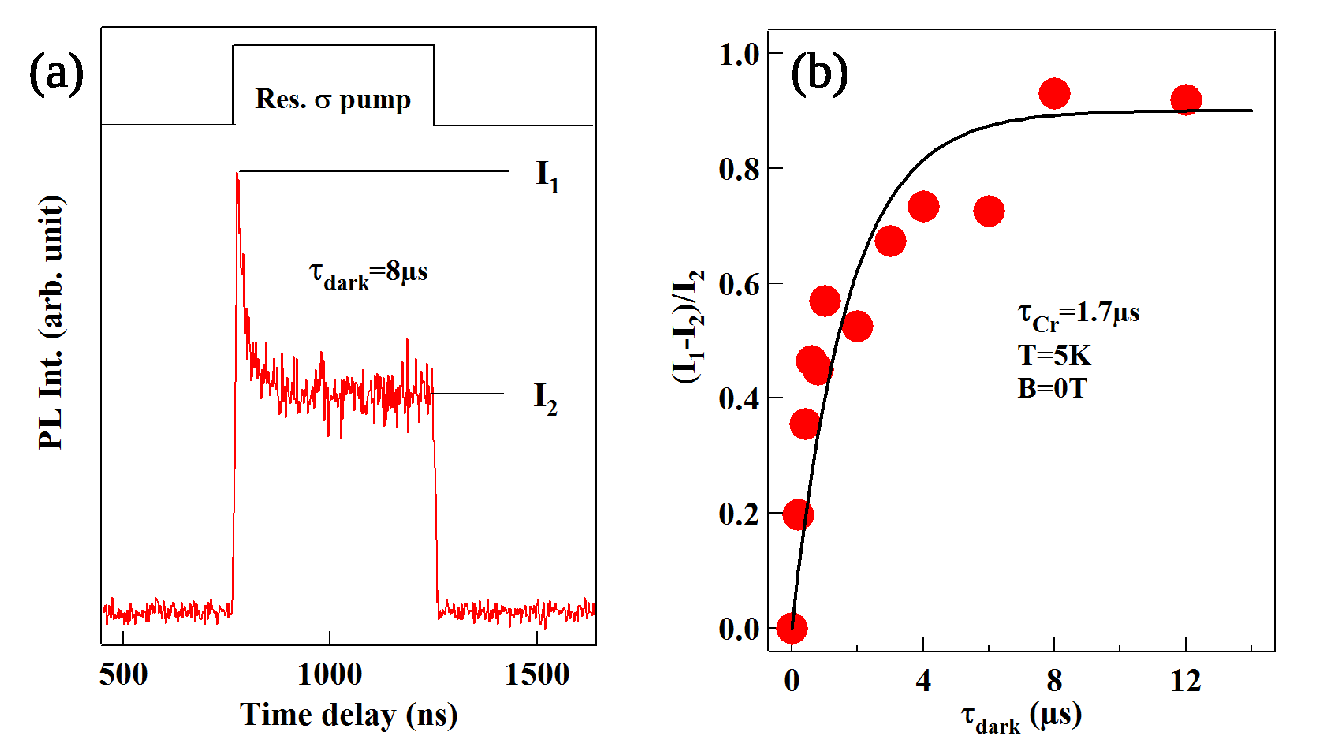
\includegraphics[width=10cm]{Pictures/RelaxDark.eps}
	\end{center}
	\caption{Dark time variation of pumping with its plot}
	\label{DarkTimeCrExp}
	\end{figure}	
	
	Lorem ipsum dolor sit amet, consectetur adipiscing elit. Curabitur tortor quam, imperdiet quis facilisis sed, fringilla a quam. Cras ante odio, hendrerit ac ante nec, cursus imperdiet urna. Mauris convallis ultricies purus, nec condimentum erat bibendum vel. Aliquam erat volutpat. Pellentesque condimentum, eros a consequat accumsan, turpis sem euismod nisi, sed fringilla quam turpis sit amet erat. Mauris dictum odio sed nisi dapibus, et molestie mauris rutrum. Praesent convallis dolor in nibh blandit bibendum. Quisque sit amet arcu consectetur lorem luctus venenatis nec quis dui. Aliquam erat volutpat. Aenean auctor elit nec tristique dignissim. Nulla massa mi, efficitur semper ex id, pretium eleifend massa. Vivamus sit amet orci scelerisque, gravida est ut, vulputate odio.

	\section{Optical control of the spin of a Cr atom}
		
		Lorem ipsum dolor sit amet, consectetur adipiscing elit. Curabitur tortor quam, imperdiet quis facilisis sed, fringilla a quam. Cras ante odio, hendrerit ac ante nec, cursus imperdiet urna. Mauris convallis ultricies purus, nec condimentum erat bibendum vel. Aliquam erat volutpat. Pellentesque condimentum, eros a consequat accumsan, turpis sem euismod nisi, sed fringilla quam turpis sit amet erat. Mauris dictum odio sed nisi dapibus, et molestie mauris rutrum. Praesent convallis dolor in nibh blandit bibendum. Quisque sit amet arcu consectetur lorem luctus venenatis nec quis dui. Aliquam erat volutpat. Aenean auctor elit nec tristique dignissim. Nulla massa mi, efficitur semper ex id, pretium eleifend massa. Vivamus sit amet orci scelerisque, gravida est ut, vulputate odio.
	
	\begin{figure}[h!]
	\begin{center}
		\includegraphics[width=10cm]{Pictures/FillingPicture.png}
	\end{center}
	\caption{Map of peak 3 and 4 under augmentation of the excitation power + line shape with plot of the splitting variation with power}
	\label{OptStarkCrExp}
	\end{figure}		
	
	Curabitur eget ipsum egestas dui viverra suscipit. Cras aliquet lacus vitae erat finibus semper. Nulla pharetra eget urna vitae sodales. Nunc faucibus velit lacus, nec ornare eros aliquet quis. Donec a orci nec sem pulvinar ultricies sit amet ut arcu. Nullam id vehicula enim, at tincidunt velit. Duis vestibulum lorem a molestie fringilla. Nullam tincidunt semper placerat. Donec nibh sem, ornare eget cursus ac, luctus sit amet eros. Phasellus eget interdum nisi. Donec mollis risus id lectus fringilla, et commodo risus iaculis. Donec at lacus sed nibh posuere posuere sit amet eget sapien. In dignissim, enim sit amet convallis fermentum, lacus nulla gravida tortor, non facilisis ex nisl sit amet augue. Maecenas eu enim condimentum, consectetur ligula vel, tincidunt nisl. Nam laoreet dictum volutpat. Donec at erat venenatis, ultrices lorem ac, vestibulum neque.
	
	\begin{figure}[h!]
	\begin{center}
		\includegraphics[width=10cm]{Pictures/FillingPicture.png}
	\end{center}
	\caption{Map of peak 3 and 4 under augmentation of the detuning + line shape with plot of the splitting variation with detuning}
	\label{StarkDetuneCrExp}
	\end{figure}	
	
	Curabitur eget ipsum egestas dui viverra suscipit. Cras aliquet lacus vitae erat finibus semper. Nulla pharetra eget urna vitae sodales. Nunc faucibus velit lacus, nec ornare eros aliquet quis. Donec a orci nec sem pulvinar ultricies sit amet ut arcu. Nullam id vehicula enim, at tincidunt velit. Duis vestibulum lorem a molestie fringilla. Nullam tincidunt semper placerat. Donec nibh sem, ornare eget cursus ac, luctus sit amet eros. Phasellus eget interdum nisi. Donec mollis risus id lectus fringilla, et commodo risus iaculis. Donec at lacus sed nibh posuere posuere sit amet eget sapien. In dignissim, enim sit amet convallis fermentum, lacus nulla gravida tortor, non facilisis ex nisl sit amet augue. Maecenas eu enim condimentum, consectetur ligula vel, tincidunt nisl. Nam laoreet dictum volutpat. Donec at erat venenatis, ultrices lorem ac, vestibulum neque.
	
	\begin{figure}[h!]
	\begin{center}
		\includegraphics[width=10cm]{Pictures/FillingPicture.png}
	\end{center}
	\caption{Detuning on 1 and 2 while exciting on 4}
	\label{DetuneDarkCrExp}
	\end{figure}	
	
	
\printbibliography

\end{document}